\documentclass[a4paper,twocolumn]{article}

\usepackage[utf8]{inputenc}
\usepackage[english]{babel}
\usepackage{graphicx}
\usepackage{caption}
\usepackage[left=2cm, right=2cm, top=2cm, bottom=2cm]{geometry}
\usepackage{amsmath}
\usepackage{listings}

\title{Panorama reconstruction using homographies}

\author{
	Sébastien Klasa - Polytech Paris-Sud\\
	\texttt{klasa.sebastien@gmail.com}
}

\date{28 October 2018}

\begin{document}
	
\maketitle

\begin{abstract}
	As part of the image processing course in the fifth year of engineering school Polytech Paris-Sud, this project aims to reconstruct a panorama from several photographs by finding homographies between pairs of images. As the purpose of the project is to understand the construction of panoramas, we implemented all algorithms ourselves. However, we use the OpenCV library to open, save and display images. We divided the project into four parts: detecting corners using the FAST detector, pairing them, finding the homography and finally constructing the panorama by transforming the images.
\end{abstract}

\section{FAST detector}

The first step of constructing a panorama is to find corners (i.e. interest points) in two overlapping images in a way that some of the corners corresponds to the same regions in both images. There are many methods of corner detection and we chose FAST (Features from Accelerated Segment Test) for its easy implementation. I implemented the naive version of the algorithm: for each pixel $p$ a circle of radius 3 is considered, if in this circle exists at least $n$ contiguous pixels which intensities are all higher or all lower than the intensity of $p$, it is labeled as a corner. I use a threshold $t$ such as for a pixel $x_i$ in the circle, if $I(p) - t \le I(x_i) \le I(p) + t$ then $x_i$ and $p$ have the same intensity. By formalizing, a pixel $p$ is a corner if one of this two conditions is met:

\begin{align*}
\exists S | \forall x \in S, I(x) \le I(p) - t\\
\exists S | \forall x \in S, I(x) \ge I(p) + t
\end{align*}

where $S$ is a set of $n$ contiguous pixels in the circle.
\\

I tested my implementation by comparing my results to the FAST detector implemented in OpenCV using the parameters $n = 12$ and $t = 50$ (see figures \ref{my_fast} and \ref{opencv_fast}). We can see in those two images that the same corners are detected but my implementation detects less of them: this is probably due to a different method of non-maxima suppression. Another interesting comparison can be the execution time: for this image, OpenCV found corners in less than 5 ms and my implementation took about 500 ms. The execution time of my algorithm is longer because I implemented the naive version, which could be improved by examining 4 example pixels and rejecting non-corners before searching the contiguous pixels.

\begin{figure}[h]
	\centering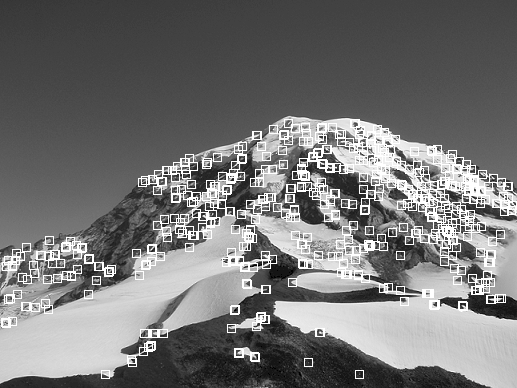
\includegraphics[width=0.5\textwidth]{images/my_fast.png}
	\caption{Result of my implementation of the FAST detector.}
	\label{my_fast}
\end{figure}

\begin{figure}[h]
	\centering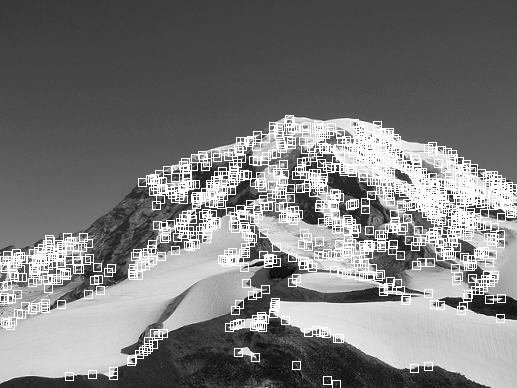
\includegraphics[width=0.5\textwidth]{images/opencv_fast.png}
	\caption{Result of the OpenCV FAST detector.}
	\label{opencv_fast}
\end{figure}

\section{Pairing}

The second step of contructing a panorama is to find common structures in two overlapping images. To do that, we find corners in both images and search for pairs of corners that are similar (that comes from the same region in the two images). In this project I use my implementation of the FAST detector decribed in the previous section to find the corners.
\\

For each image, I create a list of $9 \times 9$ squares centered on the corners, the pixels in these squares are my features. To pair them, for each corner in the first image, I compute the sum of squared distances (SSD) with corners of the second image and then keep the pair that have the lower distance. For two corners $c_1$ and $c_2$, the SSD is defined as follows:

$$
SSD(c_1, c_2) = \sum_{x = 1}^{9} \sum_{y = 1}^{9} \left[c_1(x, y) - c_2(x, y)\right]^2
$$

where $c(x,y)$ is the intensity of the pixel $(x,y)$ in the square around the corner $c$.
\\

To make this method more robust to global variations of intensity (e.g. photographs with different expositions), I replaced the SSD by a zero-mean sum of squared distances where the mean of a corner is substracted from it before computing the distance :

$$
SSD(c_1, c_2) = \sum_{x = 1}^{9} \sum_{y = 1}^{9} \left[(c_1(x, y) - \bar{c_1}) - (c_2(x, y) - \bar{c_2})\right]^2
$$

where $\bar{c} = \frac{1}{9\times9} \sum_{x = 1}^{9} \sum_{y = 1}^{9} c(x,y)$.
\\

Another improvement that I made to this algorithm is that for a corner $c_1$ in the first image, I keep the best matching corner $c_{2-best}$ only if the distance between $c_1$ and $c_{2-best}$ is much smaller that the distance between $c_1$ and the second best matching corner $c_{2-second}$:

$$
SSD(c_1, c_{2-best}) \le \frac{SSD(c_1, c_{2-second})}{2}
$$

I finally optimized the result of this algorithm by using the married pairing strategy: I run the algorithm twice, first pairing corners from image 1 to image 2, then from image 2 to image 1. I finnaly keep only pairs of corners that were paired reciprocally. The final result is shown is figure \ref{pairing}, for this example I ran the FAST detector with a high threshold to detect less corners, making the figure \ref{pairing} more readable.

\begin{figure*}
	\centering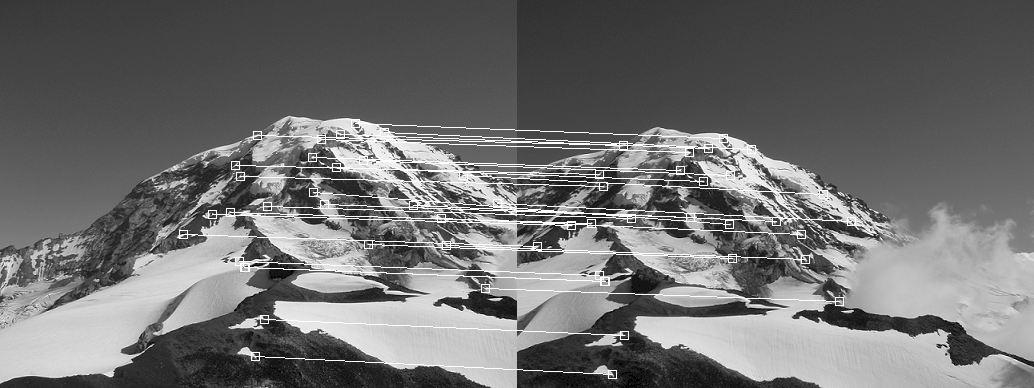
\includegraphics[width=\textwidth]{images/pairs.png}
	\caption{Result of the pairing algorithm.}
	\label{pairing}
\end{figure*}

\end{document}